\section{Simulation Analysis}

To be sure of the values obtained in \ref{sec:theo}, we made use of Ngspice, a more stable version of the Berkeley SPICE, which is an "open source spice simulator for electric and electronic circuits", as stated in \cite{ngsite}. The code used was the following, \\

{\itshape
TCFELab1 \par
.options savecurrents \\\par

Vin 1 4 5.03847501972 \par
Id 0 6 1.01674167773m \par

$V_{dumb}$ CFP1 7 0 \\\par

R1 2 1 1.03994439216k \par
R2 3 2 2.07923431764k \par
R3 2 5 3.06168544529k \par
R4 4 5 4.09516986362k \par
R5 5 6 3.00136467001k \par
R6 4 CFP1 2.03324628446k \par
R7 7 0 1.02216788331k \\\par

Gb 6 3 2 5 7.01505323139m \par
Hc 5 0 $V_{dumb}$ 8.37372457746k \\\par

.op\par
.control\par
    run\par
    print all\par
.endc\par
.end
}

\vspace{10px}
The first line of this code is the title of the simulation itself, which is followed by the option to save currents, a command that allows the program to, when printing all the variables, also print the currents flowing in every component of the circuit. Then, \textit{Vin} and \textit{Id} are the $V_a$, $I_d$ corresponding to what is shown in Fig. \ref{fig:nodal_scheme}. $V_{dumb}$ is a dumb voltage source that was introduced for a specific reason that will be later explained. In this simulation, we chose node 8 to be GND, which, by Ngspice standards, has to be named node 0.\\

After this, all the resistances were declared in the form \textit{R<name> <n+> <n-> <value>}, where n+ and n- mean the positive and negative nodes of the electronic component, according to the schematics shown in Fig.\ref{fig:polos}. \\

\begin{figure}[h]
    \centering
    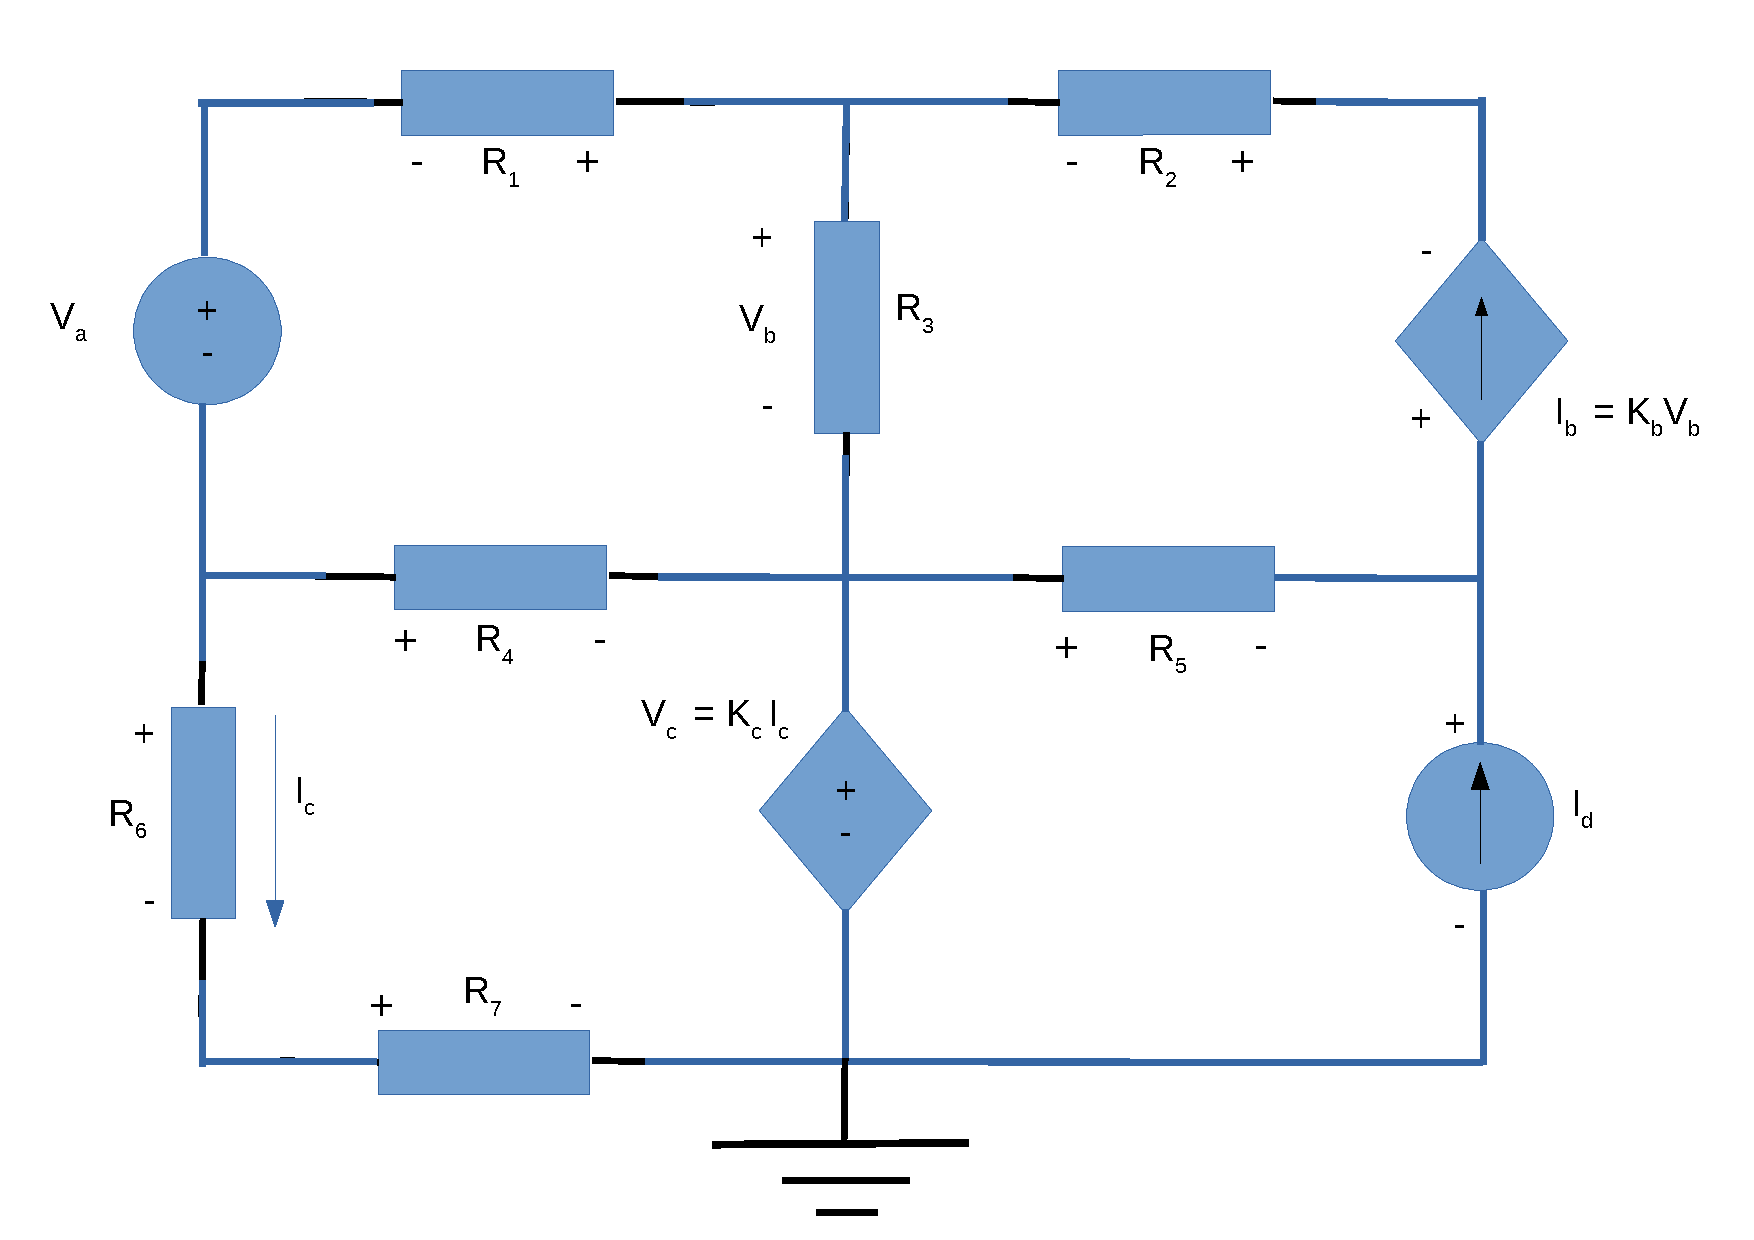
\includegraphics[width = 0.7\linewidth]{esquemacpolos.pdf}
        \caption{\textit{Representation of the convention used to the Ngspice simulation. In the figure above, one can see the conventioned positive and negative terminal for each branch}}
    \label{fig:polos}
\end{figure}

Afterwards, $Gb$ and $Hc$ stand for the voltage-controlled current source $I_b$ and current-controlled voltage source $V_c$ respectively. The first two parameters received by $Gb$ are its positive and negative nodes as expected and then the two nodes where it should calculate the corresponding potential. For $Hc$, the third parameter is $V_{dumb}$ which, as promised, is a voltage source that was introduced for the single purpose that current-controlled voltage sources in \textit{Ngspice} take as a third parameter only voltage sources through which the current in question is flowing through. Thus, because the purpose is to retrieve $I_c$, a dumb voltage source was added after $R_6$, creating a new node that was called CFTP1, which is where $R_6$ then connects. To not alter the circuit at all, the actual induced voltage by $V_{dumb}$ is 0V, thus CFTP1 and node 7 are in short circuit, i.e., the circuit does not "see" $V_{dumb}$. At last, inside \textit{control}, the simulation is ran and everything is printed out, giving the following output:\\\par


\begin{table}[H]
\setlength{\tabcolsep}{10pt}
\renewcommand{\arraystretch}{1.1}
\centering
    \begin{tabular}{||c|c||}
    \hline
    Name & Current/Voltage [A/V]\\
    \hline
    @cb[i] & 0.000000e+00\\ \hline
@ce[i] & 0.000000e+00\\ \hline
@q1[ib] & 7.022567e-05\\ \hline
@q1[ic] & 1.404513e-02\\ \hline
@q1[ie] & -1.41154e-02\\ \hline
@q1[is] & 5.765392e-12\\ \hline
@rc[i] & 1.411536e-02\\ \hline
@re[i] & 1.411536e-02\\ \hline
@rf[i] & 7.022567e-05\\ \hline
@rs[i] & 0.000000e+00\\ \hline
v(1) & 0.000000e+00\\ \hline
v(2) & 0.000000e+00\\ \hline
base & 2.254108e+00\\ \hline
coll & 5.765392e+00\\ \hline
emit & 1.411536e+00\\ \hline
vcc & 1.000000e+01\\ \hline

    \end{tabular}
\vspace{0.2 cm}
\caption{Values for several variables declared in the .net file.}
\label{max}
\end{table}


\vspace{10px}

The values obtained were expected in some way given to the results obtained in the theoretical analysis and that were presented in the last section. \\

However, due to \textit{machine epsilons} and related things, some decimal places might be a bit different. The main cause of this is that Ngspice also uses, if possible, nodal analysis. Thus, for solving matrix \ref{eqnodos}, one has to be aware that inverting a 9x9 or 7x7 matrix will introduce a significant margin of error, which explains the registered difference in the results obtained.
